\section*{Informations générales}
 
\begin{table}[h]
\centering
	\begin{tabularx}{16.8cm}{|X|X|}
	\hline
	\rowcolor{gray!40} Numéro de l'opportunité & Type de l'opportunité \\
	\hline
	001 & Acquisition d'un serveur gratuit pour le livrable \\
	\hline
	\end{tabularx}
\end{table}

\begin{table}[H]
\centering
	\begin{tabularx}{16.8cm}{|X|X|X|}
	\hline
	\rowcolor{gray!40} Date & Visa du \RQ & Visa du \CP \\
	\hline
	 07/12/15 & pgpic & pgpic \\
	\hline
	\end{tabularx}
\end{table}

\begin{table}[h]
\centering
	\begin{tabularx}{16.8cm}{|X|X|X|X|}
	\hline
	\rowcolor{gray!40} Pilote & Activité WBS & Compte WBS & Phase d'apparition \\
	\hline
	 \Matthieu & Suivre les Risques et Opportunités & 1.2.3.2 & Dès le début du PIC\\
	\hline
	\end{tabularx}
\end{table}

\section*{Description de l'opportunité}

\subsection*{Résumé}
	L'opportunité lié à l'acquisition d'un serveur gratuit permettrait de pouvoir déployer notre livrable et de mettre en place le service pour le client, sans contrainte budgétaire.
	
\subsection*{Analyse des causes}
	voir figure.

\subsection*{Criticité}

\begin{table}[h]
\centering
	\begin{tabularx}{16.8cm}{|>{}X|X|}
	\hline
	Bénéfice & 4\\
	\hline
	Probabilité & 1\\
	\hline
	Criticité & Important\\
	\hline
	\end{tabularx}
\end{table}
\newpage

\section*{Actions}
\subsection*{Actions proactives}

%\begin{table}[h]
\centering
	\begin{longtable}{|p{7cm}|p{7cm}|}
	\hline
	\rowcolor{gray!40} Numéro de cause & Actions préventives \\
	\hline
	 1 & \begin{itemize}
	 	\item Formation sur les démarches nécessaires à la constitution d'un dossier de mécénat
	 \end{itemize} \\
	\hline
	2 &
	\begin{itemize}
		\item Recherche d'un hébergeur
		\item Comparaison des offres
		\item Étudier leur susceptibilité à accepter un mécénat
	\end{itemize} \\
	\hline
	3 & \begin{itemize}
		\item Constitution d'un dossier de mécénat
	\end{itemize} \\
	\hline
	4 & \begin{itemize}
		\item Discuter de la possibilité avec l'unité P3
		\item Faire une demande auprès de l'INSA
	\end{itemize} \\
	\hline
	5 & \begin{itemize}
		\item Faire une demande de mécénat auprès de l'hébergeur
		\item Faire connaître l'Unicef à l'hébergeur (plaquette, etc.)
		\item Discuter des avantages pour l'hébergeur à accepter le mécénat
	\end{itemize} \\
	\hline
	6 & \begin{itemize}
		\item Faire une demande auprès de l'Unicef France
	\end{itemize} \\
	\hline
\end{longtable}
%\end{table}

\section*{Décision de clôture}
Par le \CP{} et le pilote du risque.
\begin{table}[h]
\centering
	\begin{tabularx}{16.8cm}{|X|X|}
	\hline
	\rowcolor{gray!40} Date de clôture & Raison de la clôture \\
	\hline
	  & \\
	\hline
	\end{tabularx}
\end{table}

\section*{Historique des modifications}
\begin{table}[h]
\centering
	\begin{tabularx}{16.8cm}{|X|X|}
	\hline
	\rowcolor{gray!40} Date & Modification \\
	\hline
	  & \\
	\hline
	\end{tabularx}
\end{table}
\newpage


\begin{figure}
	\centering
	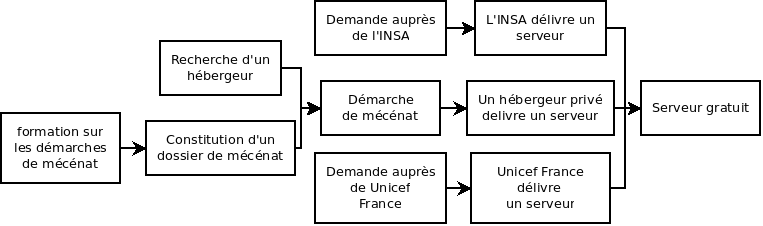
\includegraphics[scale=0.35]{images/AnalyseOpportunite_nPourquoi_FDO001.pdf}
\end{figure}